\documentclass[10pt,aps,twocolumn,secnumarabic,balancelastpage,amsmath,amssymb,nofootinbib,floatfix]{revtex4}

%%\usepackage{setspace}
%%\setstretch{1.25}
\usepackage{graphicx}      % tools for importing graphics
%\usepackage{lgrind}        % convert program code listings to a form 
                            % includable in a LaTeX document
%\usepackage{xcolor}        % produces boxes or entire pages with 
                            % colored backgrounds
%\usepackage{longtable}     % helps with long table options
%\usepackage{epsf}          % old package handles encapsulated postscript issues
\usepackage{bm}            % special bold-math package. usge: \bm{mathsymbol}
%\usepackage{asymptote}     % For typesetting of mathematical illustrations
%\usepackage{thumbpdf}

\usepackage[colorlinks=true]{hyperref}  % this package should be added after 
                                        % all others.
                                        % usage: \url{http://web.mit.edu/8.13}

\renewcommand{\baselinestretch}{1.0} 

\begin{document}
\title{Photoelectrons, Statistics and Pulse Analysis}
\author{MIT Department of Physics}
\email{nodbody\@mit.edu}
\homepage{http://web.mit.edu/8.13/}
\date{\today}
%\affiliation{MIT Department of Physics}

%-------------------------------------------------------------------------------
\begin{abstract}
  In this experiment, we learn to use the oscilloscope and investigate the photo-electron effect and its statistical behaviour. In the first part of the experiment, we acquaint ourselves with basic functionality of the scope and learn to manipulate different waveforms from a function generator. In the second part, we use an LED and a photo-multiplier tube to determine the probability distribution of the number of photons hitting the photo-multiplier in a given time interval. By changing the rate of events, we explore both Poisson and Gaussian distributions. We also investigate the probability distribution of time intervals between successive events.

{\bf This year this experiment will have to rely on recorded data. The description has been expanded to include a more thorough analysis of the recorded pulses. Please take into account that you will not be able to perform the data recording yourself, so please skip over the instructions for the recording. It is nevertheless useful to read those as it makes it more clear what the data is that has been recorded.}
\end{abstract}

\maketitle

%-------------------------------------------------------------------------------
\section*{Preparatory Questions}

\begin{enumerate}
\item In a sentence or two, describe the function of the following functions on the oscilloscope a) trigger b) time base and offset c) input channels with AC-DC coupling.
\item If a green photon ($\lambda$ = 532~nm) penetrates the glass window of the photo-multiplier tube and hits the bi-alkali layer ($\phi$ = 2.1~eV) on the inside emitting a photo-electron, what is the maximum energy it could have? Compare this energy to the energy of electron due to acceleration by $\sim$ 300~V between the cathode and the first dynode.
\item You detect a triangular signal with a peak of 20~mV and a time base of 20~ns. Calculate the gain if the signal is terminated by a 50~Ohm resistor. 
\item What is the most likely time difference between two consecutive events? Evaluate this probability for two random events at a rate of 100~events/$\mu$s to be within 20~ns.
\item What is the uncertainty on the mean of a Gaussian distribution? How does it improve when adding more data?
\item Using a computer program or online tool, create a 100-event, Poisson distributed synthetic histogram with mean, $\mu$ = 2. What does this distribution look like? What does the variance appear to be?

% \item {\bf Challenge Question - you may need to have taken 8.044 to do this one!}: Noise is thermal electrons that have been liberated from the photocathode, which then enter the photomultiplier tube and are amplified, just like an event. Give a rough estimate of the noise rate at 297~K, for a monolayer 2" diameter cathode, where the atoms have a density of 1 atom/nm$^2$. Hint: use the Maxwell-Boltzmann distribution. 

\end{enumerate}

%-------------------------------------------------------------------------------
\section{Theory}

\subsection{The Photoelectric Effect}

The photoelectric effect was discovered by Heinrich Hertz~\cite{buchwald1994} in 1887 who observed that when ultraviolet light fell on a negative electrode, electricity flowed to the anode. This experimental observation prompted Albert Einstein~\cite{einstein1905} to study the idea proposed by Max Planck in 1900 that electromagnetic radiation carries energy in 'packets' we call photons, where each photon carries energy equal to $h\nu$~\cite{planck1900}. In 1905, using the experimental data on the photoelectric effect, Einstein published a paper to re-iterate the idea that light travels in discrete quantized packets of energy~\cite{einstein1905}. 

\begin{figure*}
  \centering
  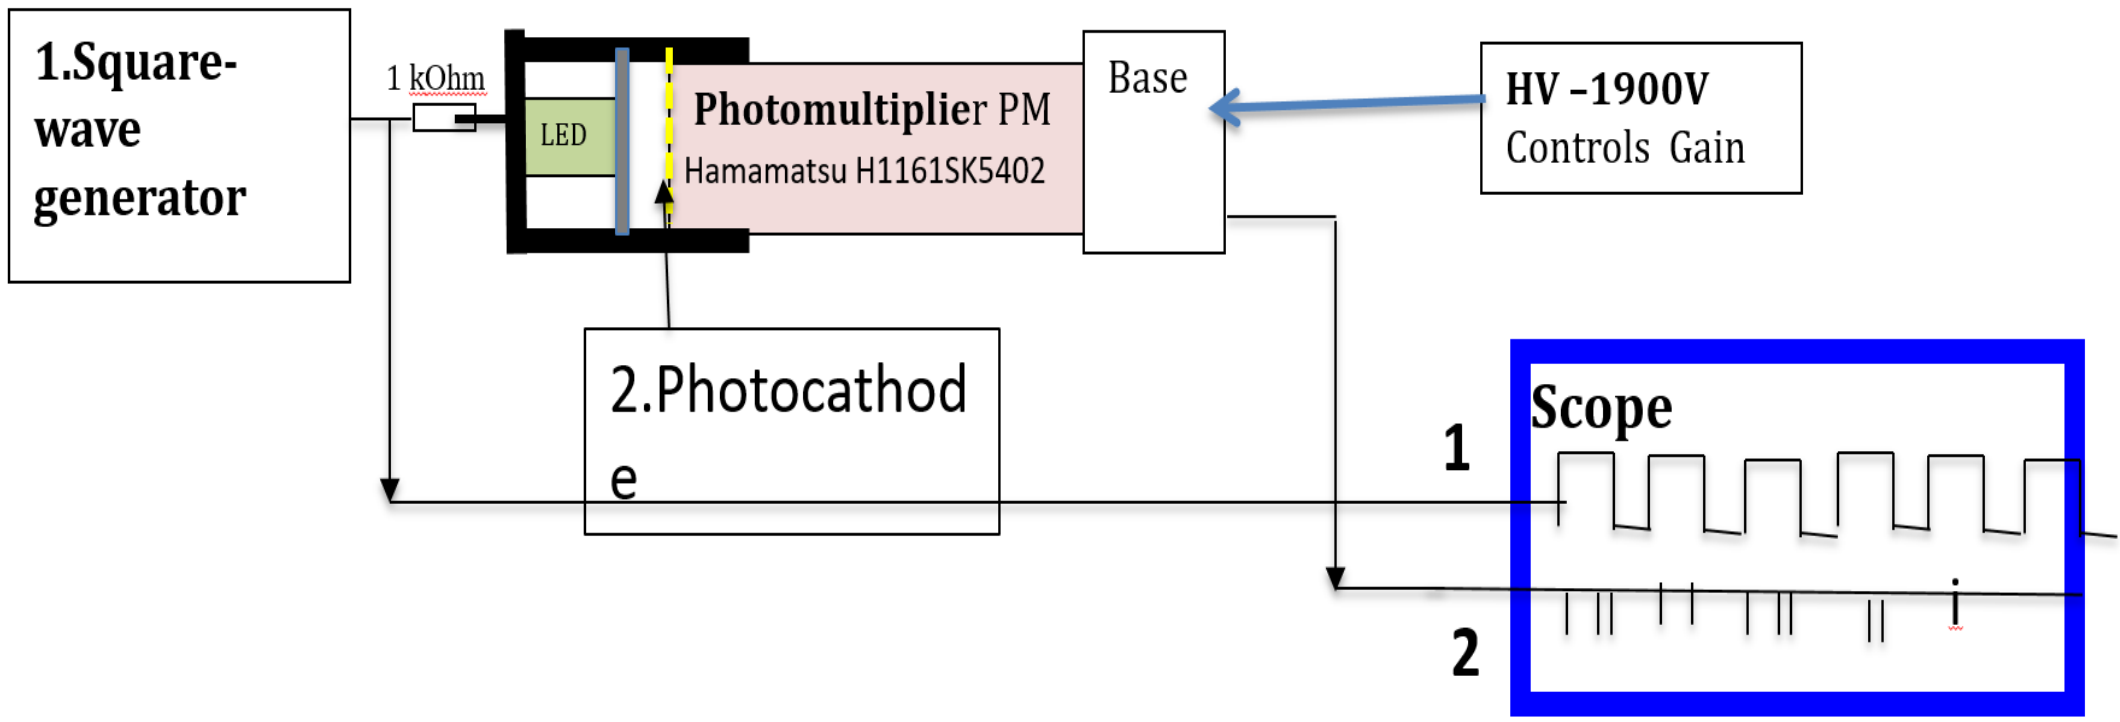
\includegraphics[width=1.0\linewidth]{figs/apparatus1.png}
  \caption{The schematic of the experimental setup}
  \label{fig:apparatus1}
\end{figure*}

The photoelectric effect is the emission of electrons when light hits a material. Electrons emitted by this process are called photoelectrons. Each material has a characteristic work function $\phi$ (electron binding energy) which is the amount of energy required to remove an electron from its surface. If the incoming photon has an energy higher than the work function $\phi$, the electron will be ejected with a maximum kinetic energy given by
%%
\begin{equation}
  K = h\nu - \phi
\end{equation}
%%
where $h$ is the Planck's constant with a value of $6.626\times10^{-34}$ Js or $4.135\times10^{-15}$ eVs.

\subsection{Poisson Statistics}

The Poisson probability distribution describes the probability of a given number of events occurring within a fixed time and/or space interval if these events occur with a given average rate and are independent~\cite{WP-poisson-distribution}. Common examples of Poisson distribution involve the number of decay events from a radioactive source, number of typos on a page of this document, number of meteors larger than a meter striking Earth in a year, number of calls received by a call center in an hour {\it etc.} Can you think of some processes that do not follow a Poisson distribution? Do you think the number of airplanes arriving at Boston Logan Airport in a five-minute interval is an example of Poisson distribution? 

The probability distribution of a Poisson random variable $X$ representing the number of events occurring in a given time interval or space interval is given by
%%
\begin{equation}
  P(X) = \frac{e^{-\lambda} \lambda^{x}}{x!} \ ,
\end{equation}
%%
where $\lambda$ is the average number of events occurring in a fixed interval of time. In the Poisson distribution, both the expected value and variance are equal to $\lambda$. 
\begin{equation}
  E(X) = \lambda ~~~~\text {and} ~~~~ \text{Var}(X) = \sigma^2 = \lambda \ .
\end{equation}

%-------------------------------------------------------------------------------
\section{Goals for the experiment}

For the photoelectron experiment we have the following goals:
\begin{enumerate}
\item Learn how to operate an oscilloscope.
\item Learn about the photoelectric effect.
\item {\bf Learn about Poisson and Gaussian distributions.}
\end{enumerate}

%-------------------------------------------------------------------------------
\section{Experimental Setup}

The components of this experiment include:
\begin{enumerate}

\item Green LED: The green LED takes voltage pulses from the function generator, and when the voltage is above a certain threshold, it produces green photons ($\lambda$ = 560 nm). These photons pass through a black attenuating cloth. Those that make it through the attenuator impinge onto the photocathode. 

\item Photocathode: Photons incident on the photocathode cause electrons to be emitted via the \textbf{photoelectric effect}. These electrons are drawn to the first dynode of the photomultiplier tube. 

\item Photomultiplier Tube (PMT): The photomultiplier tube amplifies the signal of a single electron, increasing the number of electrons by several orders of magnitude via the use of dynodes. The dynodes have a low work function and easily emit secondaries that hit the next dynode. The PMT is connected to the High Voltage (HV) supply, which provides $\sim$1877~V to the PMT. This voltage should not be changed throughout the experiment. What does the high voltage from the HV supply affect?

\begin{figure}
  \centering
  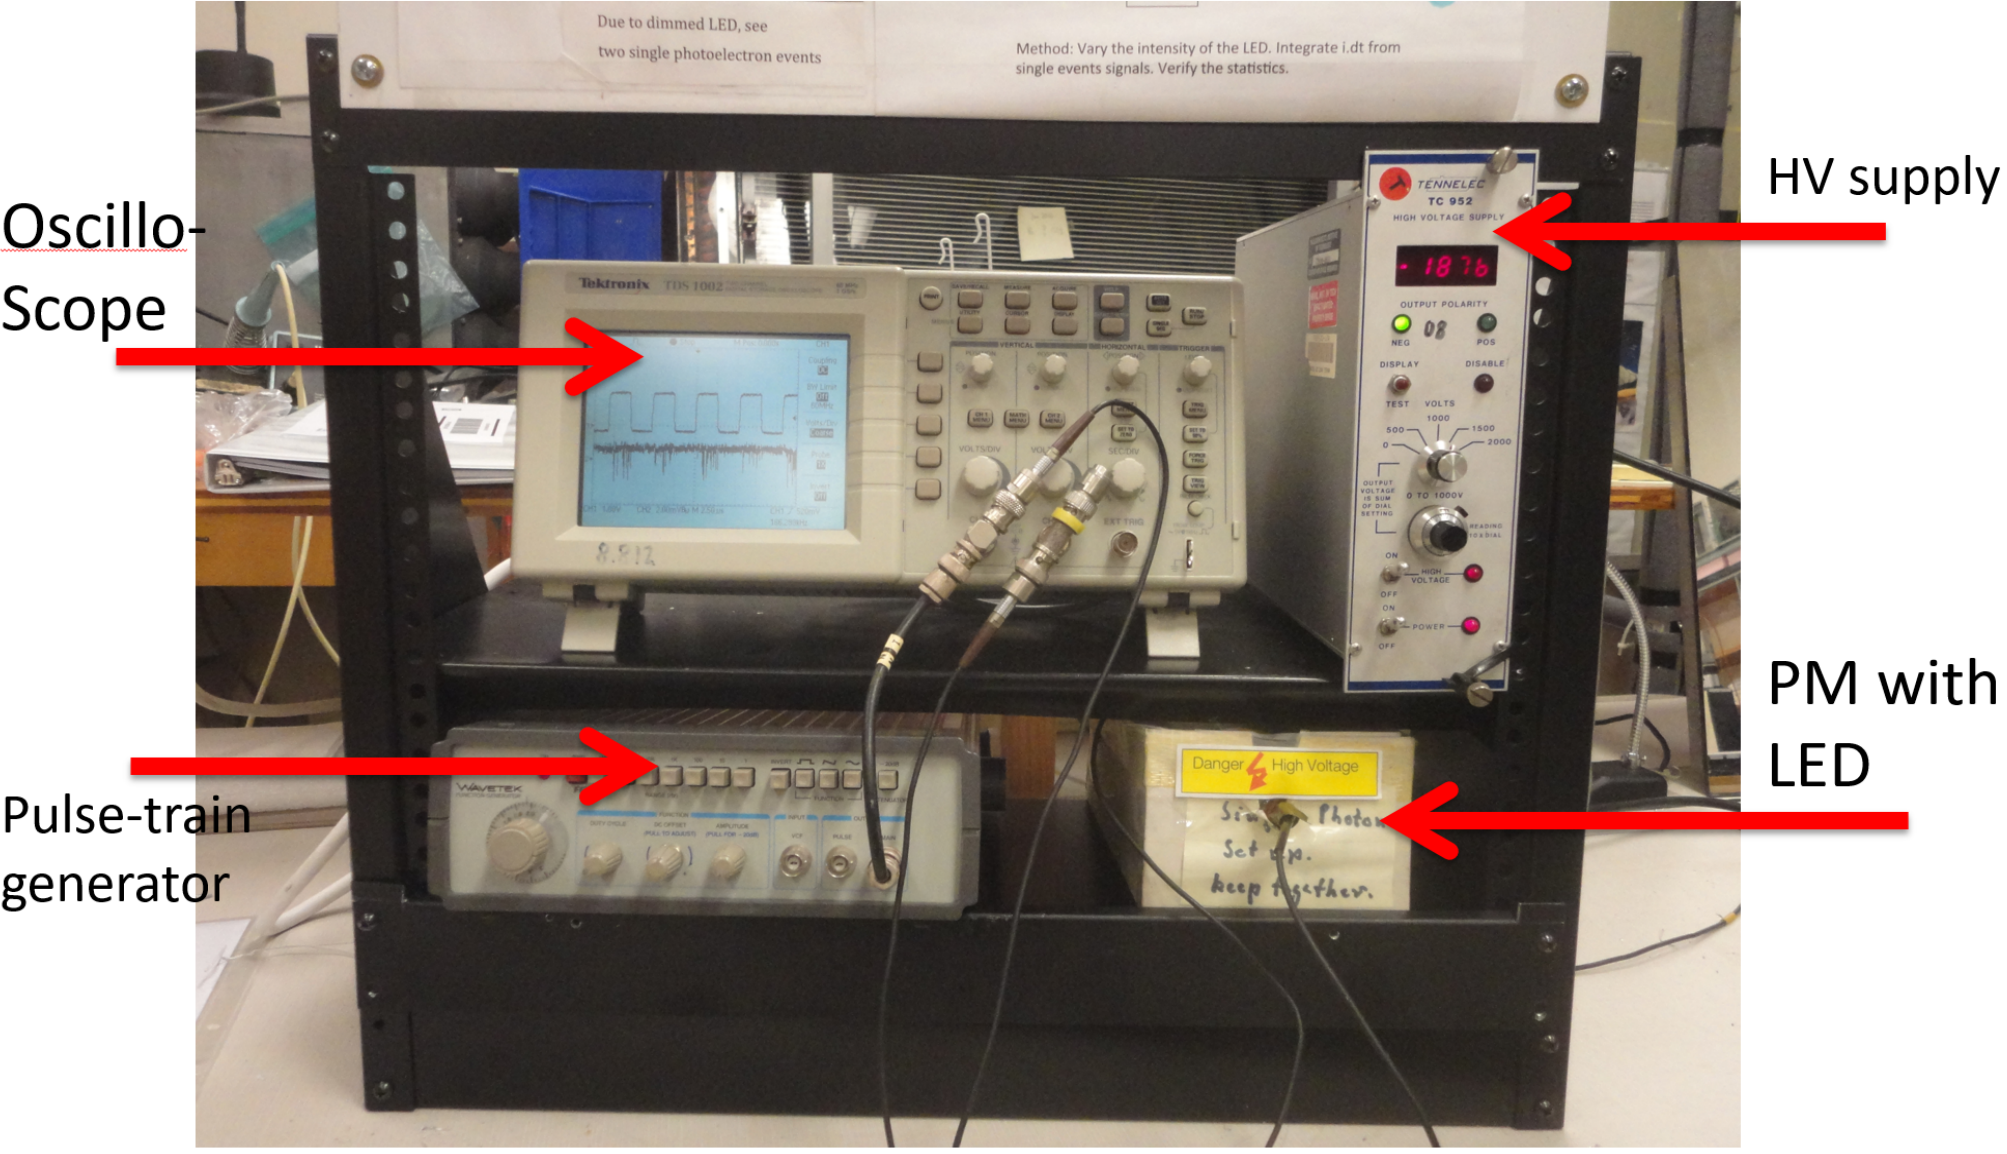
\includegraphics[width=1.0\linewidth]{figs/apparatus2.png}
  \caption{The setup of apparatus in the lab}
  \label{fig:apparatus2}
\end{figure}

\item Function Generator: The function generator outputs a periodic function whose shape, amplitude, and period can be adjusted. For this experiment, we will be using the function generator to create square pulses with a period of about 5~$\mu$s.

\item Oscilloscope: The oscilloscope displays signals from the generator and the PMT, allowing for visual diagnostics and quantitative analysis. The function generator and the PMT should be connected to the oscilloscope (see Figure \ref{fig:apparatus1}) \cite{tds2000}. 

\end{enumerate}

%-------------------------------------------------------------------------------
\section{Experiment}

\subsection{Scope exercises}

For the oscilloscope exercise please follow the steps outlined below carefully. The hardware can be damaged if not operated properly.

\begin{enumerate}
\item Switch on the oscilloscope, the function generator and the HV supply. The voltage should read $\sim$1877~V. Please do not change the voltage for the rest of the experiment. 

\item Check that function generator output is sent to channel 1 on the scope and the output of the PMT is sent to channel 2 with a 50~Ohms terminator. This terminator is quite important, can you think of a reason why?

\item Ensure that the function generator is sending in square-waves and the range is set to `100~K'. If there is no signal on the scope or if the signal appears frozen, press the `RUN/STOP' button on the top right corner. 

\item Move the `TRIGGER LEVEL' until a stable signal is achieved. Can you understand what the `TRIGGER' does?

\item You should now be able to see a train of square-wave pulses and the photo-electron signal. Find the period and amplitude of the square-wave pulses and write them down in your notebook. 

\begin{figure}
  \centering
  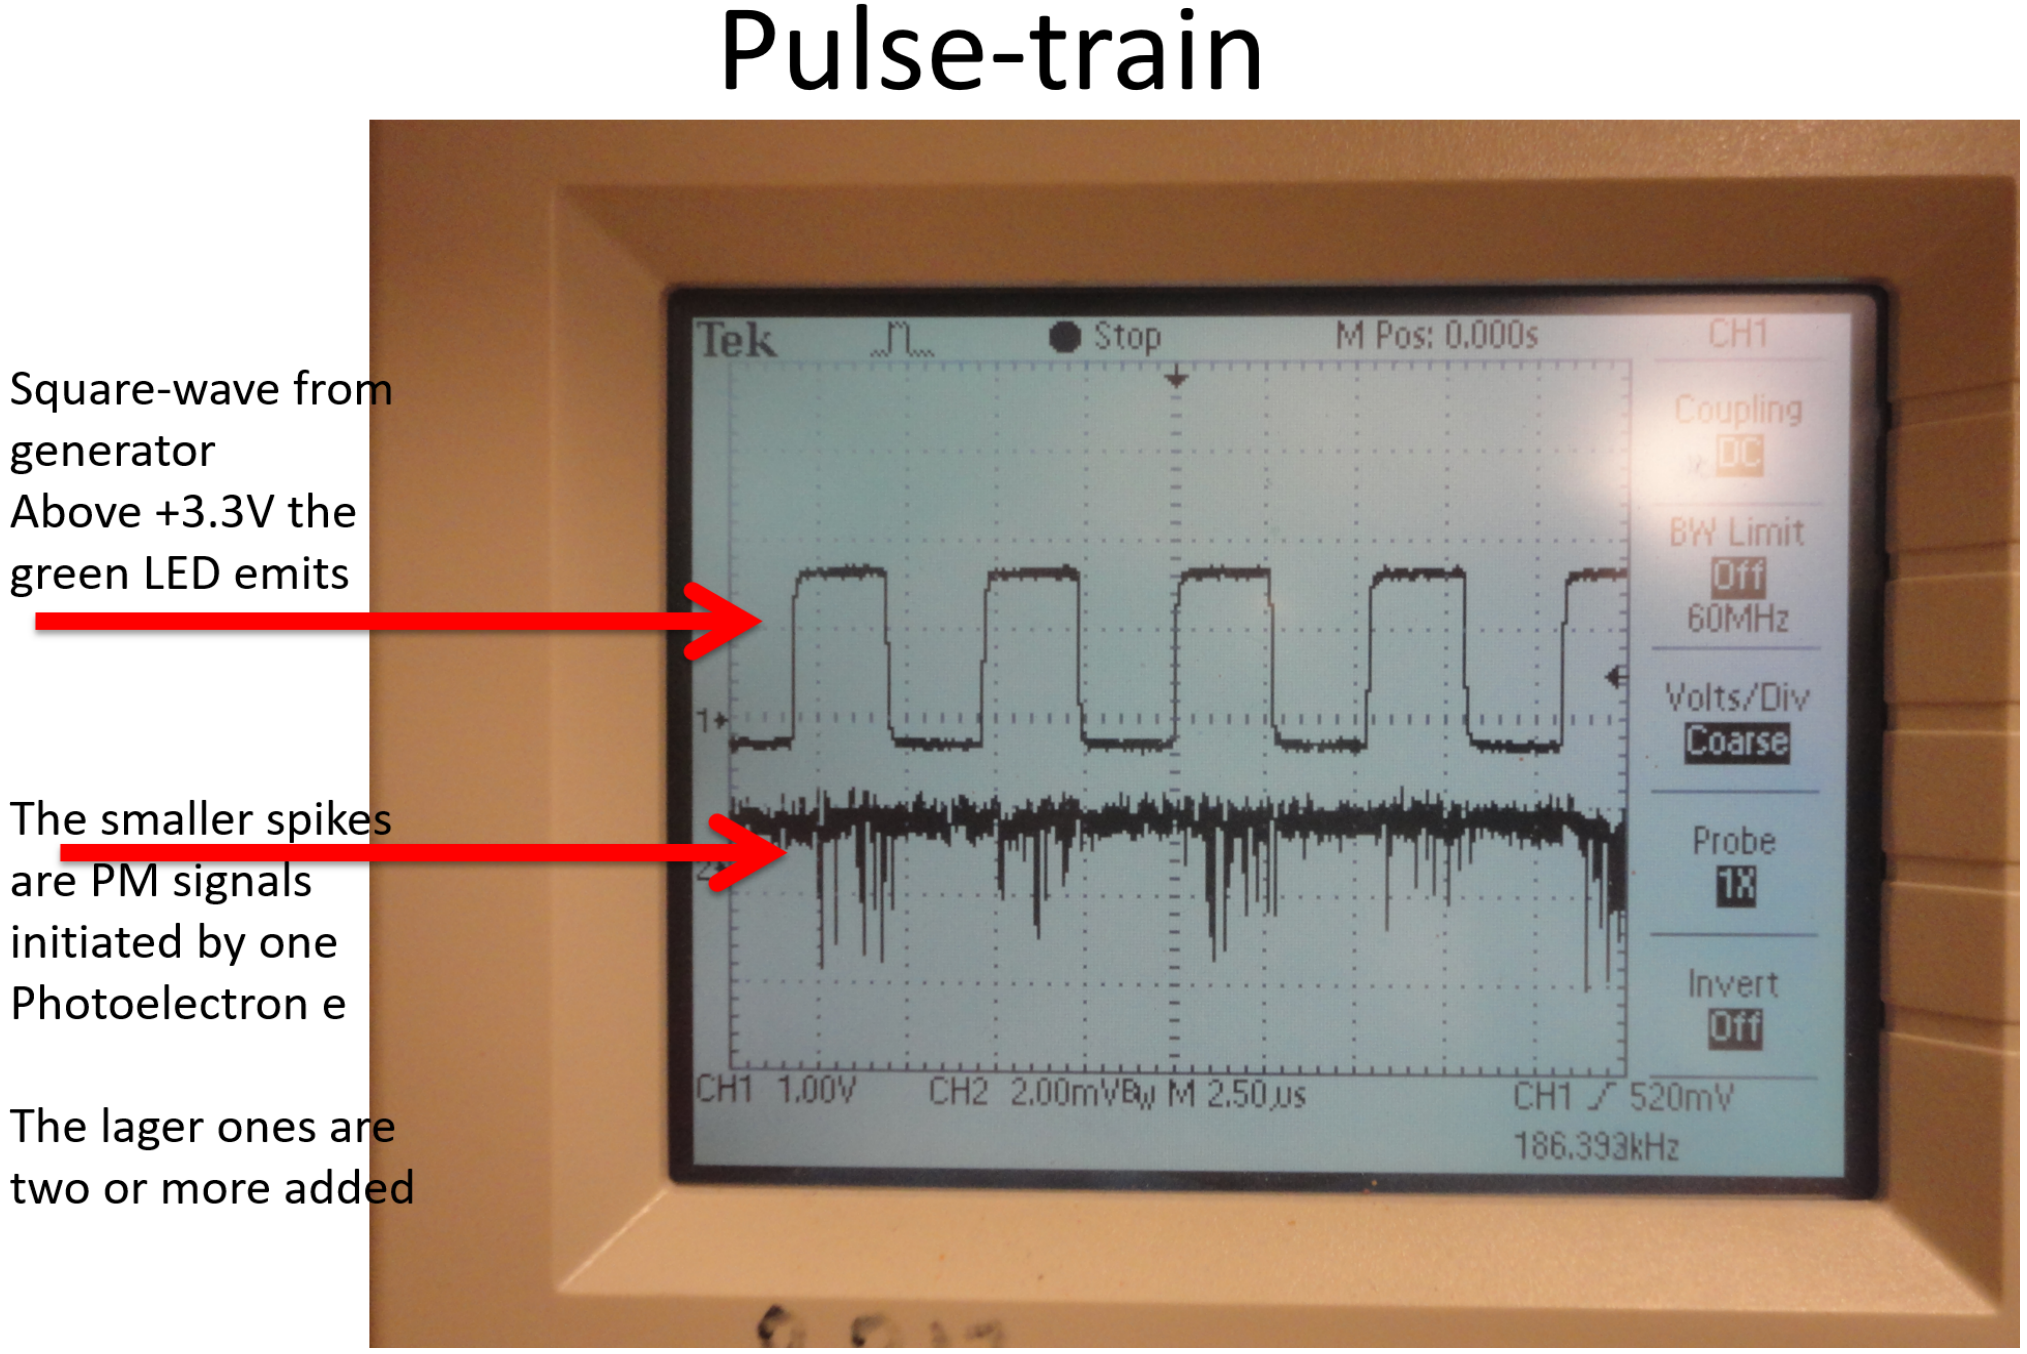
\includegraphics[width=1.0\linewidth]{figs/pulsetrain.png}
  \caption{The pulse train expected to be seen on the oscilloscope.}
  \label{fig:pulsetrain}
\end{figure}

\item Play around with the `VERTICAL' position and scale for both channel 1 and channel 2 on the scope. Does changing the position affect the period and amplitude of the signal? Does changing scale affect the period and amplitude? 

\item Now do the same for `HORIZONTAL' position and scale. How does that affect the period and amplitude of the signal? Which channel's signal does it affect?

\item Try changing to a different waveform on the function generator. Can you explain what happens? Now change the amplitude on the function generator. What do you see?

\item Why is the signal from the PMT upside down (negative)?

\item Using `RUN/STOP' to record the trace on a USB stick. You will find more instructions on collecting data using a USB stick in the user manuals for scopes available right next to the scope. Print out your trace and verify that you got what you wanted. 

\item Go back to generating square waveform from the function generator. Zoom into the time domain using the horizontal scale until the scale reads on the order of 20~ns. Ensure that you are triggering on channel 2 with a falling slope. By adjusting the position knobs, you should be able to see a single peak in detail. 

\item Assuming that the signal shape can be approximated by a triangle, compute the gain of the PMT as you did for the preparatory problem. Do not forget about the 50~Ohms terminator! Repeat the calculation a few times. You should observe that $Q$ varies by $\sim$~30\% depending on where the electron emerged from the photo-cathode. {\it Pro-tip: No number in experimental physics without its uncertainty! - Prof. Becker}

\end{enumerate}

\subsection{Photo-electron statistics exercises}

\begin{enumerate}

\item Pause collection of the oscilloscope, and adjust channel 2 scale (signal from PMT) until you can clearly see individual peaks. This means that you are detecting single photons and we are now ready to record data.

\item Adjust the function generator's frequency until the average number of peaks per function maximum (bin) is between 1 and 5 and record 100 intervals.

%\item {\bf Use the recorded data and count the number of negative voltage peaks that are at least 10 times larger than the noise, in the corresponding time. What do you think the taller peaks signify, and how should they affect your count per bin?}

%\item {\bf Plot a histogram of the number of peaks per bin and calculate its variance. Fit both a Poisson and Gaussian distribution to the data. Qualitatively, which is a better fit?}

\item Now, adjust the oscilloscope until the average count is greater than ten and record 100 intervals.

%\item {\bf Analyze the recorded data as previously and plot another histogram and calculate the variance. Fit both a Poisson and Gaussian to this data. Qualitatively, which is a better fit?}

\end{enumerate}

%-------------------------------------------------------------------------------
\section{Reading recorded oscilloscope data}

After recording a number of intervals as described before we will proceed to a more detailed analysis of the pulse data. Therefore start by installing the software package following the instructions in Reference~\cite{cite:pulses}.

\subsection{Understanding single oscilloscope traces}
Use the data in the 'data' directory:
\begin{enumerate}
\item Select two typical but different plots of pulses and explain what the features are that you see.
\item The baseline and jitter of an oscilloscope recording is important to determine to be able to determine a signal. The baseline is the average reading that you expect with no signal being present, while the jitter is the fluctuation of the reading. Determine the baseline and the jitter for the two plots you showed in the last part. Explain what you did.
\item Fit a Landau function~\cite{cite:plandau} to the peak and determine the mean values and the corresponding uncertainties of the position, the width and the normalization of the peak. The analysis package already does this, but does not include the statistical uncertanties for each reading. Please, modify the code to include the uncertainties and compare the results with ones where no uncertainties are included. Calculate the $\chi^2$ and determine the number of degrees of freedom. Use those two numbers to determine the probability that the peak observed originates from the fitted landau distribution.
\end{enumerate}

\subsection{Analyze two datasets of oscilloscope traces}

The two datasets, each consisting of a number of oscilloscope recordings, are given in the directories 'data-a' and 'data-b' and have been recorded as described above. Please, perform the following tasks on each dataset.
\begin{enumerate}
\item Determine the number of photons seen per recording and produce a plot showing the distribution of the full dataset.
\item Determine the average number of photons by fitting the distribution obtained before using a Poisson and a Gaussian distribution. Please, include the statistical uncertainty.
\item Compare the result with the average rate obtained when dividing the total number of counts (sum of all recordings) by the total time (sum of the duration of all recordings).
\item Produce a picture of the cumulative averages, {\it i.e.} adding one recording after the other to the running average. Please, also keep the statistical uncertainties up to date.
\end{enumerate}


\bibliography{photon_pulses}
%-------------------------------------------------------------------------------
%\bibliographystyle{yahapj}
%\bibliography{photon_statisitics}

\begin{thebibliography}{99}

\bibitem{WP-photo-electric} 
  \href{https://en.wikipedia.org/wiki/Photoelectric\_effect}{Wikipedia: Photoelectric effect}

\bibitem{WP-poisson-distribution}
  \href{https://en.wikipedia.org/wiki/Poisson\_distribution}{Wikipedia: Poisson distribution},
  \href{https://towardsdatascience.com/the-poisson-distribution-and-poisson-process-explained-4e2cb17d459}%
       {Towards data science web site.}

\bibitem{buchwald1994}
  J.Z.~Buchwald.
  ``The Creation of Scientific Effects'',
  \href{https://press.uchicago.edu/ucp/books/book/chicago/C/bo3636276.html}%
       {The University of Chicago Press, Book, 1994}

\bibitem{einstein1905}
  A.~Einstein,
  ``\"Uber einen die Erzeugung und Verwandlung des Lichtes betreffenden heuristischen Gesichtspunkt,''
  \href{http://users.physik.fu-berlin.de/~kleinert/files/eins\_lq.pdf}%
       {Annalen der Physik Vol. {\bf 322}, Issue 6 (1905) 132-148.}, and
  A.~Peppard,
  ``Einstein's Proposal of the Photon Concept-a Translation of the Annalen der Physik Paper of 1905,''
  \href{https://aapt.scitation.org/doi/10.1119/1.1971542}%
       {American Journal of Physics, Volume {\bf 33}, Issue 5 (1965) 367-374}

\bibitem{planck1900}
  M.~Planck,
  ``Zur Theorie des Gesetzes der Energieverteilung im Normalspectrum,''
  \href{https://archive.org/stream/verhandlungende01goog#page/n247/mode/2up}{Verhandlungen der Deutschen Physikalischen Gesellschaft 2 (1900) 237–245}, and
  D. ter Haar,
  ``The Old Quantum Theory,''
  \href{https://openlibrary.org/books/OL5997151M/The\_old\_quantum\_theory}{Pergamon Press: 82 (1967) LCCN 66029628}.

\bibitem{tsitsiklis2018}
  J.~Tsitsiklis,
  ``Definition of the Poisson Process,''
  \href{https://www.youtube.com/watch?v=D\_EGYzqmapc}{MIT RES.6-012 Introduction to Probability, Spring 2018}

\bibitem{h-value}
  \href{https://physics.nist.gov/cgi-bin/cuu/Value?h}{NIST web site.}, or
  \href{http://www.physics.rutgers.edu/~abrooks/342/constants.html}{Useful constants and conversions.}

\bibitem{tds2000}
  \href{https://www.tek.com/oscilloscope/tds2000-digital-storage-oscilloscope}{Tektronics scope: TDS2000}

\bibitem{cite:pulses}
  \href{https://github.com/JLabMit/JLabExperiments/tree/master/Pulses/python}{Python package for the Pulses experiment.}

\bibitem{cite:plandau}
  \href{https://pypi.org/project/pylandau/}{Python implementation of landau function.}

\end{thebibliography}

%-------------------------------------------------------------------------------
\clearpage
\appendix
\section{More on the photomultiplier and oscilloscope}

\begin{figure}
  \centering
  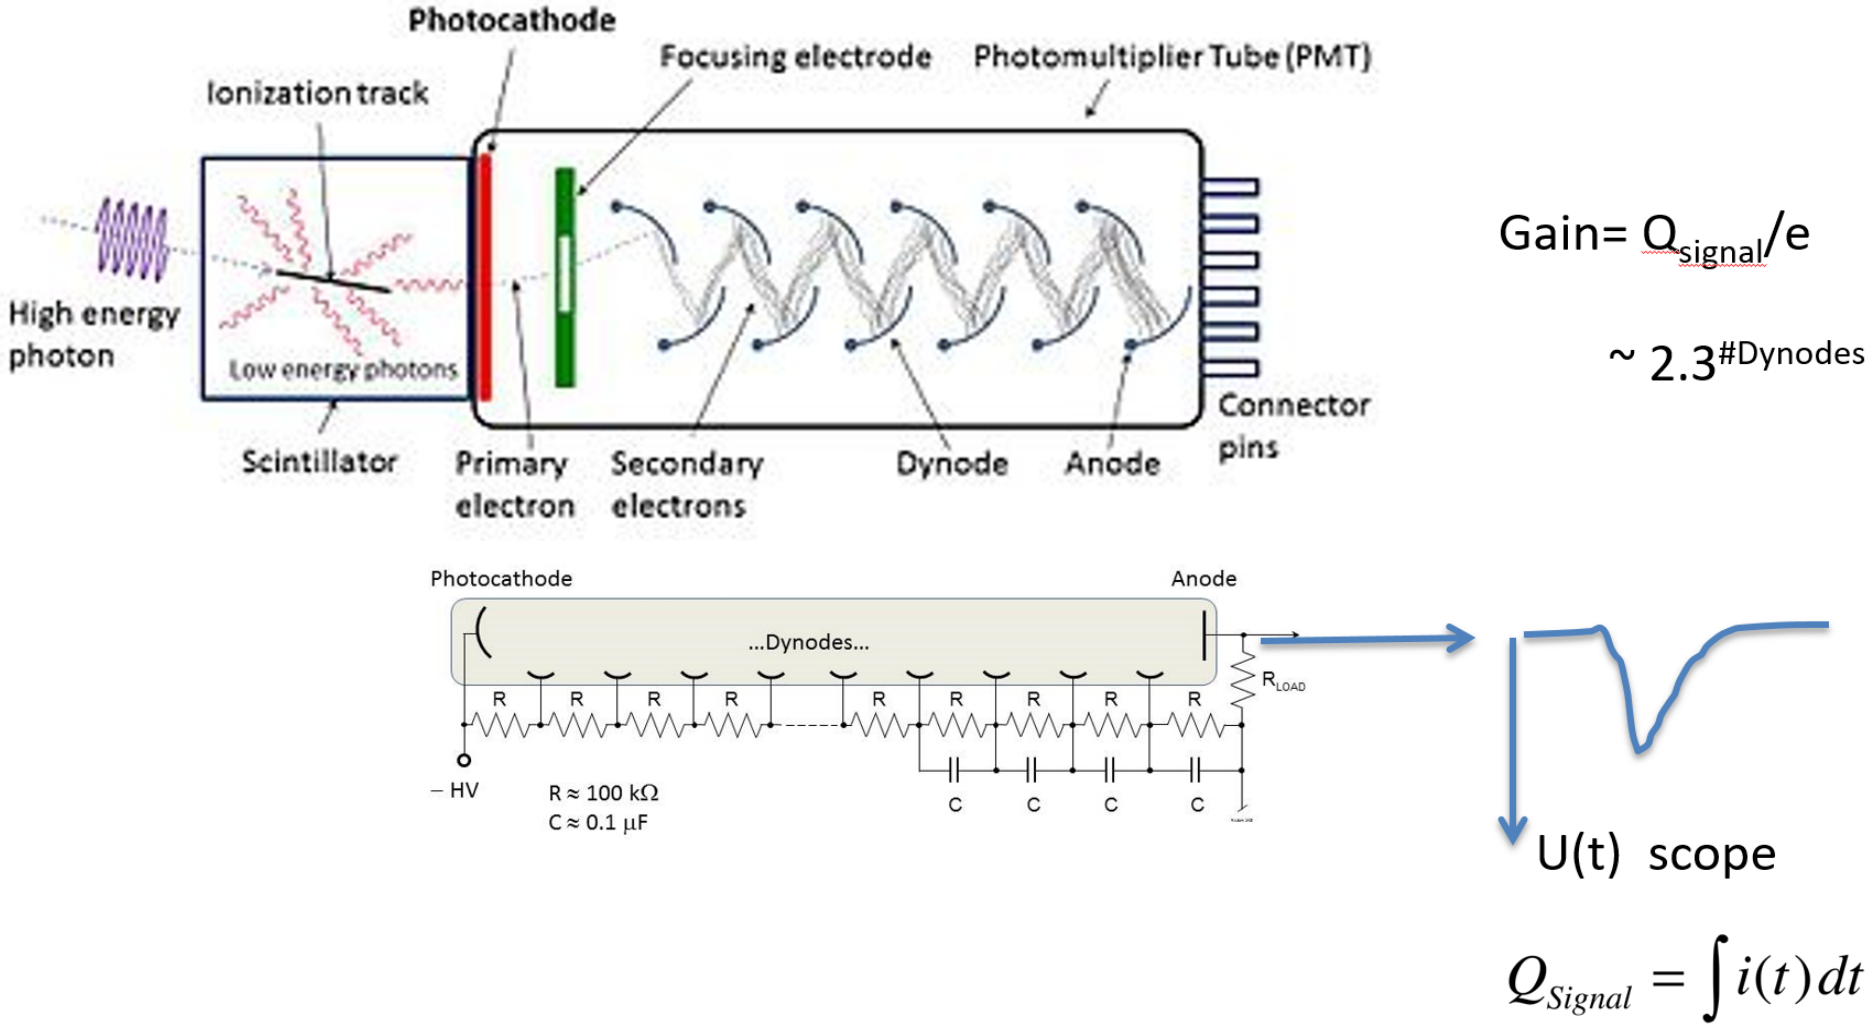
\includegraphics[width=1.0\linewidth]{figs/photomultipliertube.png}
  \caption{The schematic of signal amplification by the photomultiplier}
  \label{fig:photomultiplier-tube}
\end{figure}

\begin{figure}
  \centering
  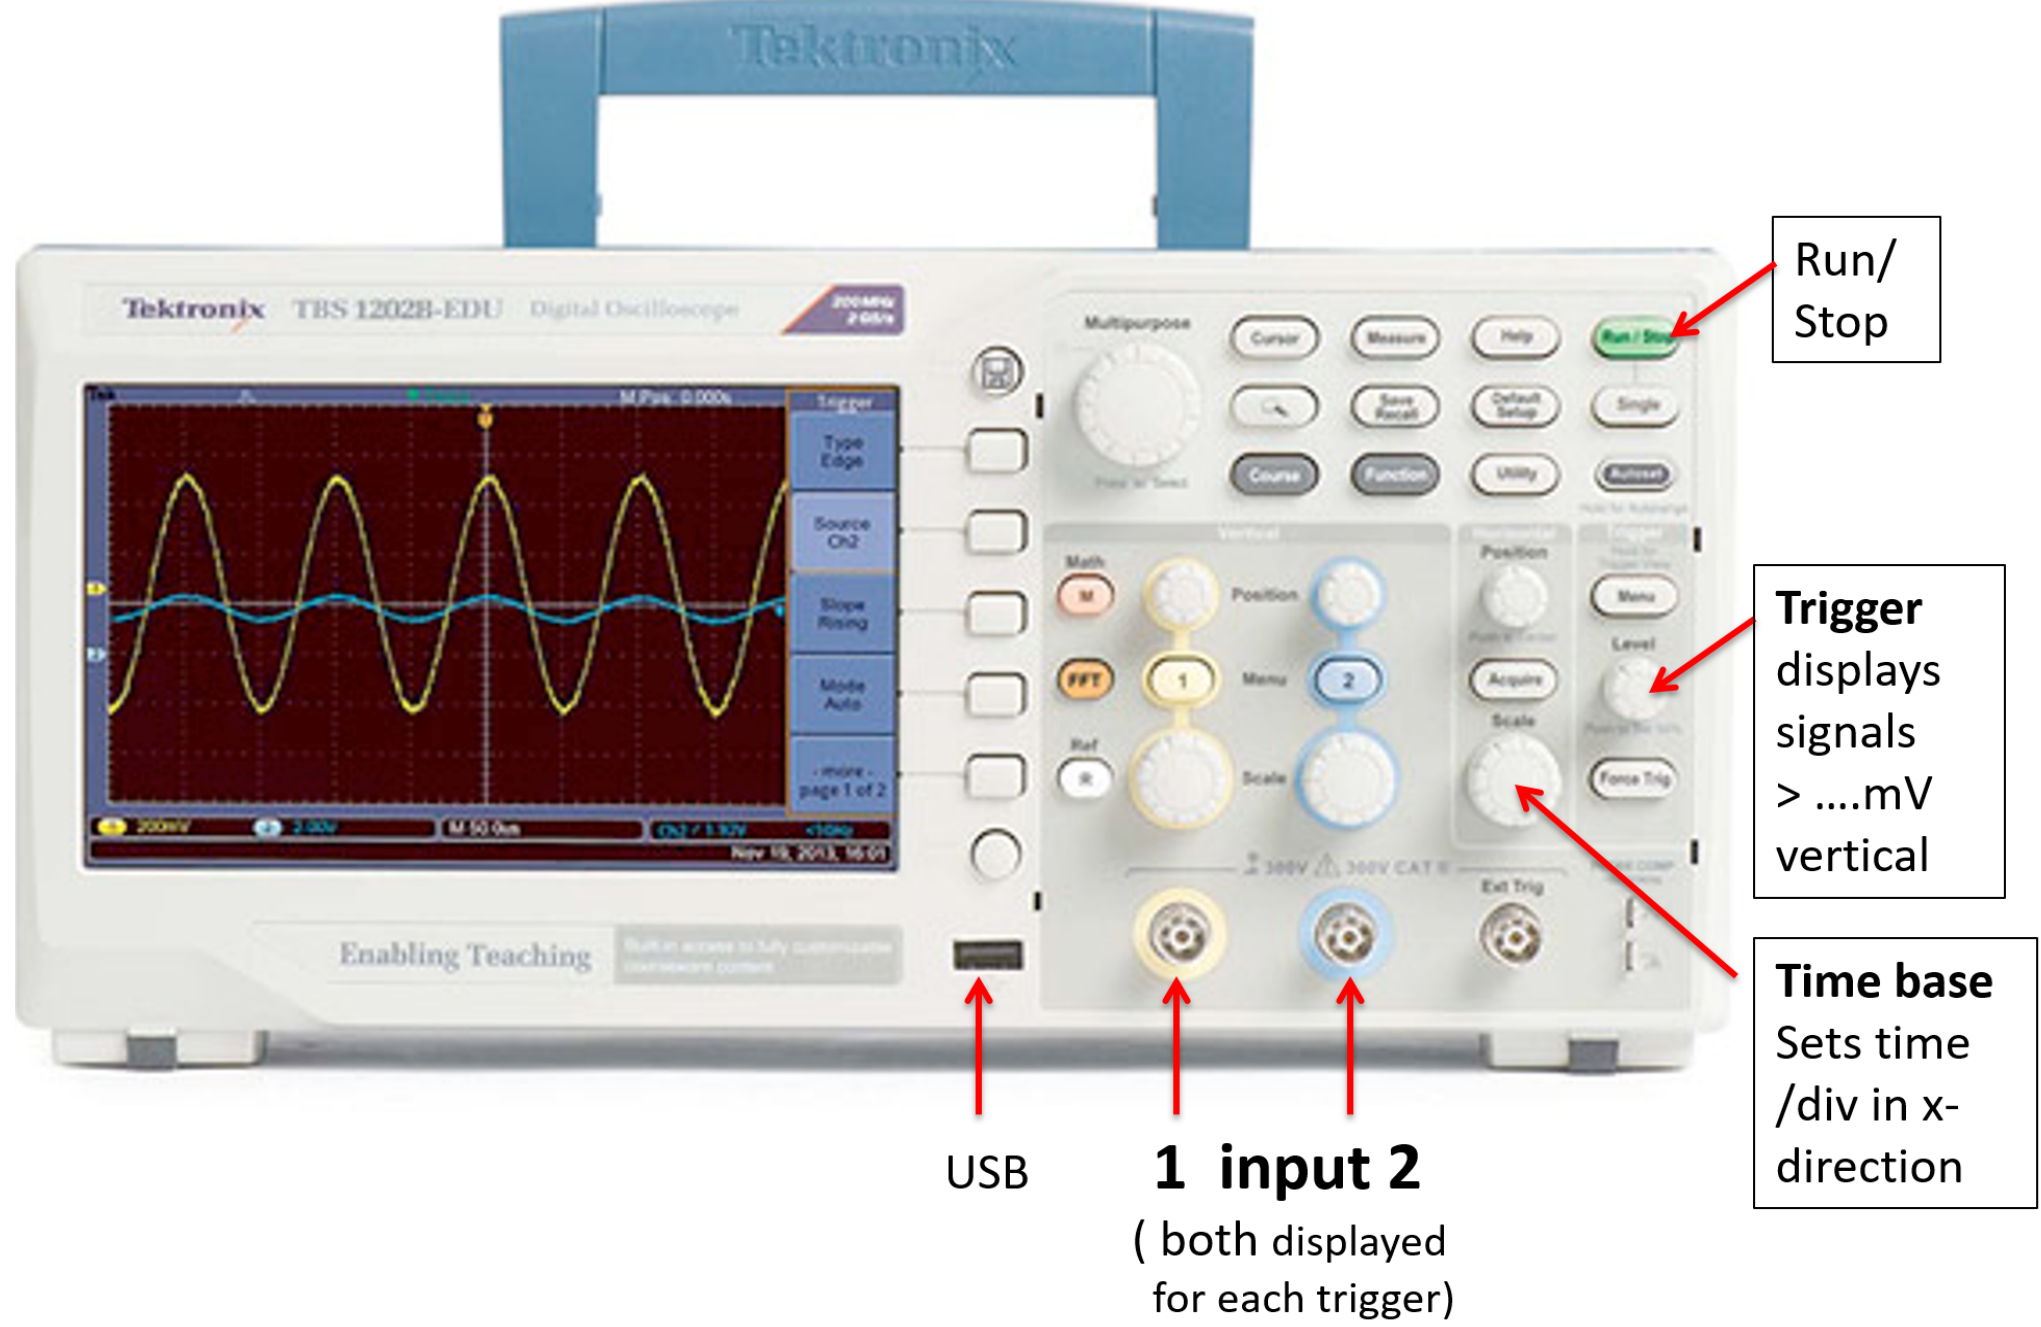
\includegraphics[width=1.0\linewidth]{figs/morescope.png}
  \caption{The different knobs and functions of the scope}
  \label{fig:morescope}
\end{figure}

To save your data into a USB stick:
\begin{enumerate}
\item Insert the USB into the port once you are ready to save the files. 
\item Press the `SAVE' button on the scope and wait until the files are all saved. 
\item The files saved into the USB stick contain a .CSV file to access your data and .JPG file which is an image of the scope output. 
\end{enumerate}

\end{document}
